\documentclass{article}
\usepackage[margin=1.5cm,bottom=2cm]{geometry}
\usepackage{fancyhdr}
\usepackage{graphicx}
\pagestyle{fancy}
\usepackage{enumitem,amssymb,amsmath}
\newlist{todolist}{itemize}{2}
\setlist[todolist]{label=$\square$}

\begin{document}
\fancyhead[L]{ 
\includegraphics[width=2cm]{au_logo.png} }
\fancyhead[R]{PHYS 2250: General Physics II}
\fancyfoot[C]{\thepage}
\vspace*{0cm}
\begin{center}
	{\LARGE \textbf{Quiz 4}}
	%\vspace{0.25cm}
	%{\Large Due: Friday, September 11}
\end{center}

\begin{enumerate}
	\item In a region of space, there is a constant electric field $\vec{E}=<800,0,0>$ N/C. Locations $A, B, $ and $C$ are given:
	\begin{itemize}
		\item $\vec{A}=<-0.5,0,0>$ m
		\item $\vec{B}=<0.5,0,0>$ m
		\item $\vec{C}=<0.5,-0.5,0>$ m
	\end{itemize}

	Calculate $\Delta V$ along each of the following paths:
	\begin{enumerate}
		\item From $A$ to $B$
		\item From $B$ to $A$
		\item From $B$ to $C$
		\item From $A$ to $C$
	\end{enumerate}
	
	\begin{figure}[ht!]
		\centering
		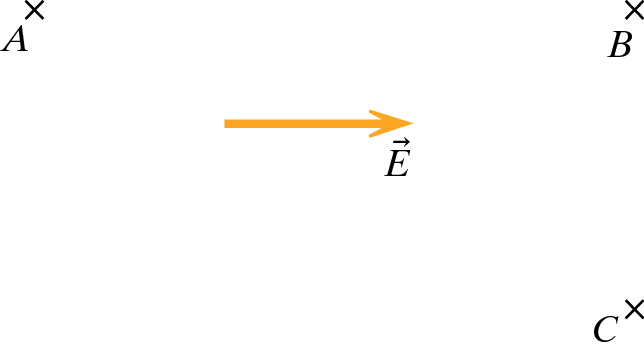
\includegraphics[width=5cm]{Ch16jpegs/fig16_65.jpg}
	\end{figure}
\vspace{7cm}
\item At a point in space the electric potential (relative to infinity) can be expressed as:
\begin{equation*}
V = 3x^2 -4y + z^3
\end{equation*}
What is the electric field vector $\vec{E}$ at this location?
\end{enumerate}

\end{document}